\documentclass{beamer}
\usepackage[brazil]{babel}
%\usepackage[latin1]{inputenc}
\usepackage[utf8x]{inputenc} 
%\usepackage[all]{xy}
\PrerenderUnicode{ç}
\usepackage{algorithmic}

\setbeamercovered{transparent=5}

\usetheme{Marburg}

\title{Escalonamento de times de futebol: Propriedades especiais do algoritmo \textit{HAP-pattern}}

\author{Rodrigo L. M. Flores \\ \url{flores@ime.usp.br}}


\institute{Instituto de Matemática e Estatística\\Universidade de São Paulo}

\begin{document}

\date{\today}

\frame{\titlepage}

\begin{frame}
  \frametitle{Motivação: Torcidas brigam}
  \begin{figure}
    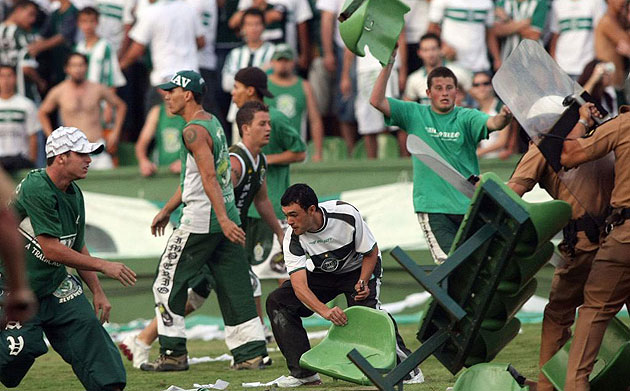
\includegraphics[scale=0.3]{torcida.jpg}
  \end{figure}
\end{frame}


\begin{frame}
  \frametitle{Motivação: TVs transmitem jogos}
  \begin{figure}
    
\includegraphics[scale=0.5]{galvao.jpg}
  \end{figure}
\end{frame}

\begin{frame}
  \frametitle{O problema}
  Dado um campeonato, com $n$ times, gerar rodadas nas quais só são permitidos $m$ jogos 
  na mesma cidade na rodada. Deve-se evitar que times joguem muitos jogos
  seguidos fora ou dentro de casa.

  \begin{itemize}
    \item Para o campeonato brasileiro, $n = 20$, $m = 2$ ($20$ times, rodada dura normalmente $2$ dias)
    \item Particularmente, para o campeonato brasileiro, $m > 1$, pois existem cidades com mais de $2$ times com torcidas expressivas 
  (São Paulo, Rio de Janeiro, Recife)
  \end{itemize}
\end{frame}

\begin{frame}
  \frametitle{Possíveis soluções}
  Problema é NP-difícil!
  \begin{itemize}
    \item \textbf{Força Bruta} - $2.9 \cdot 10^{130}$ combinações (impraticável)
    \item \textbf{Força Bruta sobre um padrão de jogos} - $2.4 \cdot 10^{18}$ combinações a serem testadas (muito custoso)
    \item \textbf{Força Bruta sobre apenas um pedaço de tamanho $k$ da instância} - $\binom{n}{k} \le n!$. Se $n = 20$, $k = 3$, 
    $\binom{20}{3} = 1140$ combinações. (razoavelmente praticável)
    \item Conclusão: podemos resolver os casos dos times de várias cidades e depois sortear os padrões para os outros times
  \end{itemize}
\end{frame}

\begin{frame}
  \frametitle{Algoritmo de geração de padrão de jogos}
  \begin{itemize}
    \item Algoritmo proposto no artigo \cite{holandes}
    \item Para um número ímpar de times, $0$ quebras no padrão ``casa-fora''
    \item Para um número par de times, $2n-2$ quebras no padrão ``casa-fora''
  \end{itemize}
\end{frame}

\begin{frame}[fragile]
  \frametitle{O Algoritmo para um número ímpar de times}
\begin{verbatim}
    def Generator.generate_round(n,g)
      round = [g]
      reverse = true
      (1...number_of_teams/2).each do |i|
        match = [normalize(g.first - i, n ),
                 normalize(g.last + i, n)]
        if reverse
          round << match.reverse
        else
          round << match
        end
        reverse = !reverse
      end
      return round
    end
\end{verbatim}
\end{frame}

\begin{frame}
  \frametitle{Para um número par de times}
    Executar o algoritmo para um número ímpar ($n-1$), e o time que sobrar joga com o time $n$ (alternando jogos fora e dentro de casa)
\end{frame}

\begin{frame}
  \frametitle{Resultado interessante}
  \begin{itemize}
    \item Os pares $(n/2 + 1,n)$, $(1,2)$,$(3,4)$,$(5,6)$,$\cdots$,$(n-2,n-1)$ possuem a seguinte propriedade: quando um deles joga em casa o outro joga
    fora de casa;
    \item Estratégia interessante: definir para cada par de times da mesma cidade um par destes;
    \item Utilizando esta estratégia, gerar um campeonato; 
  \end{itemize}
\end{frame}

\begin{frame}
  \frametitle{Programa}
  \begin{itemize}
    \item Código fonte disponível em \url{http://github.com/rodrigoflores/Scheduling}
    \item Aceita uma entrada de times e suas cidades
    \item Irá gerar uma tabela completa dado uma entrada de times, evitando que mais que $2$ times da mesma rodada joguem na mesma cidade
  \end{itemize}
\end{frame}

\begin{frame}
  \frametitle{Perguntas?}
\end{frame}

\begin{frame}
  \frametitle{Bibliografia}
  \bibliographystyle{amsalpha}
  \bibliography{bibliografia}
\end{frame}

\end{document}


% vim:set ts=2 expandtab:
